\documentclass[aspectratio=169,11pt]{beamer}

% Theme and color setup
\usetheme{Madrid}
\definecolor{cryptoblue}{RGB}{0,82,155}
\definecolor{cryptogold}{RGB}{247,147,26}
\definecolor{cryptogreen}{RGB}{39,174,96}
\definecolor{cryptored}{RGB}{192,57,43}
\definecolor{cryptopurple}{RGB}{142,68,173}
\definecolor{lightgray}{RGB}{245,245,245}

\usecolortheme[named=cryptoblue]{structure}
\setbeamercolor{title}{fg=white,bg=cryptoblue}
\setbeamercolor{frametitle}{fg=white,bg=cryptoblue}
\setbeamercolor{block title}{fg=white,bg=cryptoblue}
\setbeamercolor{block body}{bg=lightgray}

% Packages
\usepackage{tikz}
\usetikzlibrary{shapes,arrows,positioning,calc,chains,decorations.pathreplacing}
\usepackage{tcolorbox}
\usepackage{booktabs}
\usepackage{array}
% fontawesome5 removed - not available
\usepackage{graphicx}
\usepackage{adjustbox}

% Custom boxes
\newtcolorbox{argumentbox}[1][]{
  colback=cryptoblue!10,
  colframe=cryptoblue,
  title=#1,
  fonttitle=\bfseries,
  boxrule=1pt,
  arc=2pt
}

\newtcolorbox{quotebox}[1][]{
  colback=gray!10,
  colframe=gray!50,
  leftrule=4pt,
  rightrule=0pt,
  toprule=0pt,
  bottomrule=0pt,
  arc=0pt,
  #1
}

\newtcolorbox{casestudybox}[1][]{
  colback=cryptogold!10,
  colframe=cryptogold,
  title=#1,
  fonttitle=\bfseries,
  boxrule=1pt,
  arc=2pt
}

\newtcolorbox{objectionbox}[1][]{
  colback=cryptored!10,
  colframe=cryptored,
  title=#1,
  fonttitle=\bfseries,
  boxrule=1pt,
  arc=2pt
}

\newtcolorbox{probox}[1][]{
  colback=cryptogreen!10,
  colframe=cryptogreen,
  title=#1,
  fonttitle=\bfseries,
  boxrule=1pt,
  arc=2pt
}

% Reduce spacing
\setlength{\parskip}{0pt}
\setbeamertemplate{navigation symbols}{}

% Title information
\title[Cryptocurrency Philosophy]{The Political Philosophy of Cryptocurrency}
\subtitle{Digital Money, Decentralization, and the Future of Finance}
\author{Computing and AI Ethics}
\institute{Rochester Community and Technical College}
\date{}

\begin{document}

% Title slide
\begin{frame}
\titlepage
\end{frame}

% Slide 2: Central Questions
\begin{frame}{Central Questions}
\begin{itemize}
    \item What is money, and why does it matter who controls it?
    \item Can technology solve political and economic problems?
    \item Should individuals have financial privacy from governments?
    \item Is cryptocurrency a revolutionary innovation or a speculative bubble---or both?
\end{itemize}

\vspace{0.5em}
\begin{alertblock}{Discussion}
Have you ever used or owned cryptocurrency? What's your impression of it?
\end{alertblock}
\end{frame}

%% PART I: UNDERSTANDING MONEY AND CRYPTOCURRENCY %%
\section{Part I: Understanding Money and Cryptocurrency}

% Slide 3: What Is Money?
\begin{frame}{What Is Money? A Brief History}
Money is a \textbf{social technology}---not a natural phenomenon. It works because people \emph{believe} it works.

\vspace{0.3em}
\begin{table}[h]
\centering
\footnotesize
\begin{tabular}{@{}llll@{}}
\toprule
\textbf{Era} & \textbf{Form} & \textbf{Backing} & \textbf{Controller} \\
\midrule
Ancient & Commodity (gold, shells) & Intrinsic value & Markets \\
19th--20th C & Representative & Gold reserves & Central banks \\
Post-1971 & Fiat & Government decree & Central banks \\
2009--present & Cryptocurrency & Cryptography/code & Algorithms \\
\bottomrule
\end{tabular}
\end{table}

\vspace{0.3em}
Key transition: Nixon ended gold convertibility in 1971, ushering in the pure fiat era.

\begin{alertblock}{Discussion}
What gives money its value if it's not backed by gold?
\end{alertblock}
\end{frame}

% Slide 4: Three Functions of Money
\begin{frame}{The Three Functions of Money}
\begin{center}
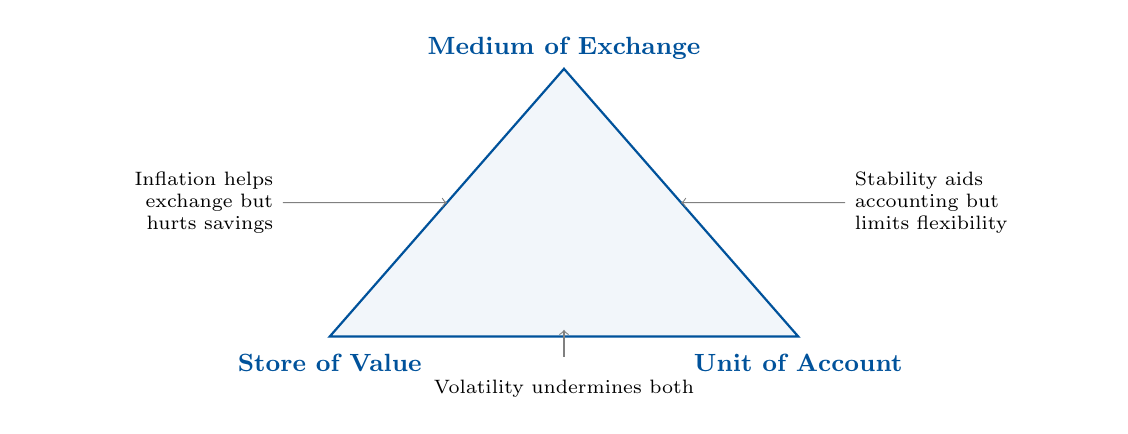
\begin{tikzpicture}[scale=0.85]
    % Triangle vertices
    \coordinate (A) at (0,4);
    \coordinate (B) at (-3.5,0);
    \coordinate (C) at (3.5,0);
    
    % Triangle
    \draw[thick, cryptoblue, fill=cryptoblue!5] (A) -- (B) -- (C) -- cycle;
    
    % Labels at vertices (in boxes)
    \node[above, font=\small\bfseries, text=cryptoblue] at (A) {Medium of Exchange};
    \node[below, font=\small\bfseries, text=cryptoblue, yshift=-3pt] at (B) {Store of Value};
    \node[below, font=\small\bfseries, text=cryptoblue, yshift=-3pt] at (C) {Unit of Account};
    
    % Edge tension labels - positioned outside with callout lines
    % Left edge (Exchange <-> Store)
    \node[left, font=\scriptsize, align=right, text width=3cm] (L1) at (-4.2,2) 
        {Inflation helps\\exchange but\\hurts savings};
    \draw[->, gray, thin] (L1.east) -- (-1.75,2);
    
    % Right edge (Exchange <-> Account)
    \node[right, font=\scriptsize, align=left, text width=3cm] (R1) at (4.2,2) 
        {Stability aids\\accounting but\\limits flexibility};
    \draw[->, gray, thin] (R1.west) -- (1.75,2);
    
    % Bottom edge (Store <-> Account)
    \node[below, font=\scriptsize] at (0,-0.5) {Volatility undermines both};
    \draw[->, gray, thin] (0,-0.3) -- (0,0.1);
\end{tikzpicture}
\end{center}

\vspace{0.1em}
\textbf{Key tension}: These functions can conflict with each other. A currency optimized for one function may fail at others.

\begin{alertblock}{Discussion}
Which function do you think is most important?
\end{alertblock}
\end{frame}

% Slide 5: How Traditional Banking Works
\begin{frame}{How Traditional Banking Works}
Banks serve as \textbf{trusted third parties} (intermediaries) in financial transactions.

\vspace{0.3em}
\textbf{Key features of modern banking:}
\begin{itemize}
    \item \textbf{Fractional reserve}: Banks lend out most deposits (keep only 10\% or less)
    \item \textbf{Ledger system}: Your ``money'' is really database entries
    \item \textbf{Central banks}: Act as ``lender of last resort'' during crises
    \item \textbf{Deposit insurance}: Government guarantees (FDIC up to \$250,000)
\end{itemize}

\vspace{0.3em}
\textbf{Vulnerabilities}: Bank runs, systemic risk, requires trust in institutions.

\begin{alertblock}{Key Example}
2008 financial crisis: What happens when trust breaks down?
\end{alertblock}
\end{frame}

% Slide 6: What Is Cryptocurrency?
\begin{frame}{What Is Cryptocurrency?}
\begin{argumentbox}[Definition]
\textbf{Cryptocurrency}: Digital currency that uses cryptography for security and operates on a decentralized network without central authority.
\end{argumentbox}

\vspace{0.3em}
\textbf{Key innovations:}
\begin{itemize}
    \item \textbf{Decentralized}: No single point of control or failure
    \item \textbf{Blockchain}: Distributed, public ledger of all transactions
    \item \textbf{Peer-to-peer}: Direct transactions without intermediaries
    \item \textbf{Cryptographic}: Secured by mathematics, not institutions
\end{itemize}

\vspace{0.3em}
\textbf{Analogy}: Email vs. postal mail---digital, direct, no central post office needed.

First and most famous: \textbf{Bitcoin} (2009)
\end{frame}

% Slide 7: How Blockchain Works
\begin{frame}{How Blockchain Works (Simplified)}
\begin{center}
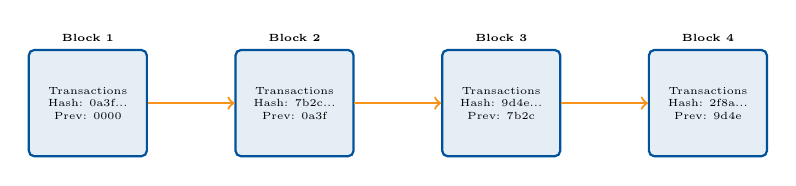
\begin{tikzpicture}[scale=0.75, transform shape,
    block/.style={rectangle, draw=cryptoblue, thick, fill=cryptoblue!10, 
                  minimum width=2cm, minimum height=1.8cm, rounded corners=2pt}]
    
    % Blocks
    \node[block] (b1) at (0,0) {};
    \node[block] (b2) at (3.5,0) {};
    \node[block] (b3) at (7,0) {};
    \node[block] (b4) at (10.5,0) {};
    
    % Block labels
    \node[above, font=\tiny\bfseries] at (b1.north) {Block 1};
    \node[above, font=\tiny\bfseries] at (b2.north) {Block 2};
    \node[above, font=\tiny\bfseries] at (b3.north) {Block 3};
    \node[above, font=\tiny\bfseries] at (b4.north) {Block 4};
    
    % Block contents
    \node[font=\tiny, align=center] at (b1) {Transactions\\Hash: 0a3f...\\Prev: 0000};
    \node[font=\tiny, align=center] at (b2) {Transactions\\Hash: 7b2c...\\Prev: 0a3f};
    \node[font=\tiny, align=center] at (b3) {Transactions\\Hash: 9d4e...\\Prev: 7b2c};
    \node[font=\tiny, align=center] at (b4) {Transactions\\Hash: 2f8a...\\Prev: 9d4e};
    
    % Chain arrows
    \draw[->, thick, cryptogold] (b1) -- (b2);
    \draw[->, thick, cryptogold] (b2) -- (b3);
    \draw[->, thick, cryptogold] (b3) -- (b4);
\end{tikzpicture}
\end{center}

\vspace{0.3em}
Each block contains transactions, timestamp, and a cryptographic hash of the previous block. Changing any block would break all subsequent hashes. Copies are stored on thousands of computers worldwide.

\begin{alertblock}{Analogy}
A shared Google Doc everyone can read and some can write to, but no one can delete or alter past entries.
\end{alertblock}
\end{frame}

% Slide 8: Proof of Work vs. Proof of Stake
\begin{frame}{Proof of Work vs. Proof of Stake}
How do we trust a system with no central authority? Different \textbf{consensus mechanisms}:

\vspace{0.3em}
\begin{table}[h]
\centering
\footnotesize
\begin{tabular}{@{}p{2.5cm}p{4.5cm}p{4.5cm}@{}}
\toprule
\textbf{Feature} & \textbf{Proof of Work (Bitcoin)} & \textbf{Proof of Stake (Ethereum)} \\
\midrule
Security method & Computational puzzles & Economic collateral \\
Energy use & $\sim$150--175 TWh/year & $\sim$0.02 TWh/year \\
Hardware & Specialized ASICs & Standard computers \\
Entry barrier & Equipment costs & Token ownership \\
Criticism & Wasteful energy & ``Rich get richer'' \\
\bottomrule
\end{tabular}
\end{table}

\begin{alertblock}{Key Point}
Both mechanisms solve the same problem: How to agree on valid transactions without a central authority.
\end{alertblock}
\end{frame}

% Slide 9: Key Features of Cryptocurrency
\begin{frame}{Key Features of Cryptocurrency}
\begin{columns}[T]
\begin{column}{0.48\textwidth}
\textbf{Technical Features:}
\begin{itemize}
    \item \textbf{Decentralized}: No single controller
    \item \textbf{Pseudonymous}: Addresses, not names
    \item \textbf{Transparent}: Public ledger
    \item \textbf{Immutable}: Can't reverse transactions
\end{itemize}
\end{column}
\begin{column}{0.48\textwidth}
\textbf{Economic Features:}
\begin{itemize}
    \item \textbf{Programmable}: Smart contracts
    \item \textbf{Limited supply}: Bitcoin caps at 21 million
    \item \textbf{Borderless}: Works globally
    \item \textbf{Permissionless}: Anyone can participate
\end{itemize}
\end{column}
\end{columns}

\vspace{0.5em}
\begin{alertblock}{Important Distinction}
Pseudonymity $\neq$ anonymity. Blockchain analysis can often identify users.
\end{alertblock}
\end{frame}

% Slide 10: Bitcoin - The Original
\begin{frame}{Bitcoin---The Original Cryptocurrency}
Created \textbf{January 3, 2009} by ``Satoshi Nakamoto'' (pseudonymous, identity unknown).

\begin{quotebox}
Genesis block message: ``The Times 03/Jan/2009 Chancellor on brink of second bailout for banks''
\end{quotebox}

\vspace{0.3em}
\textbf{Key properties:}
\begin{itemize}
    \item Maximum supply: 21 million BTC (ever)
    \item ``Halving'' every $\sim$4 years reduces new supply
    \item Emerged during 2008 financial crisis---not coincidental
    \item Current market cap: \$2+ trillion
\end{itemize}

\begin{alertblock}{The Mystery}
Satoshi disappeared in 2011. Estimated holdings: $\sim$1.1 million BTC (\$100--135 billion)---never moved.
\end{alertblock}
\end{frame}

% Slide 11: The Broader Crypto Ecosystem
\begin{frame}{The Broader Crypto Ecosystem}
``Cryptocurrency'' is a diverse ecosystem, not just Bitcoin.

\vspace{0.3em}
\begin{table}[h]
\centering
\footnotesize
\begin{tabular}{@{}lllll@{}}
\toprule
\textbf{Crypto} & \textbf{Year} & \textbf{Purpose} & \textbf{Consensus} & \textbf{Supply} \\
\midrule
Bitcoin (BTC) & 2009 & Digital gold & Proof of Work & 21M cap \\
Ethereum (ETH) & 2015 & Smart contracts & Proof of Stake & No cap \\
Tether (USDT) & 2014 & Stablecoin (\$1) & Centralized & No cap \\
Solana (SOL) & 2020 & High-speed & Proof of Stake & No cap \\
\bottomrule
\end{tabular}
\end{table}

\vspace{0.3em}
\textbf{Other categories}: DeFi (decentralized finance), NFTs (non-fungible tokens), DAOs (decentralized autonomous organizations), thousands of ``altcoins.''

\begin{alertblock}{Discussion}
Is the diversity of the crypto ecosystem a strength or weakness?
\end{alertblock}
\end{frame}

% Slide 12: Case Study - Satoshi Nakamoto
\begin{frame}{Case Study: Satoshi Nakamoto and the Cypherpunk Vision}
\begin{casestudybox}[The Cypherpunk Movement (1990s)]
Privacy advocates, cryptographers, and libertarians who believed: ``Privacy is necessary for an open society in the electronic age.'' Key figures: Timothy May, Eric Hughes, Nick Szabo, Hal Finney.
\end{casestudybox}

\vspace{0.3em}
\textbf{Prior attempts}: DigiCash (1989), b-money (1998), bit gold (2005)---all failed.

\textbf{Satoshi's breakthrough}: Solved the ``double-spending problem'' without a trusted third party using blockchain and proof of work.

\textbf{The mystery}: Satoshi communicated only via email/forums, disappeared in 2011, holds $\sim$\$100+ billion in BTC that has never moved.

\begin{alertblock}{Discussion}
Does it matter that we don't know who created Bitcoin?
\end{alertblock}
\end{frame}

%% PART II: THE CASE FOR CRYPTOCURRENCY %%
\section{Part II: The Case FOR Cryptocurrency}

% Slide 13: Political Philosophy Behind Crypto
\begin{frame}{The Political Philosophy Behind Cryptocurrency}
Cryptocurrency is \textbf{not politically neutral}---it embodies specific values.

\vspace{0.3em}
\textbf{Primary influences}: Libertarianism, Austrian economics, cypherpunk ideology.

\textbf{Key thinkers}: Friedrich Hayek (\emph{Denationalization of Money}, 1976), Murray Rothbard.

\begin{quotebox}
``I don't believe we shall ever have a good money again before we take the thing out of the hands of government... all we can do is by some sly roundabout way introduce something that they can't stop.''\\
\hfill---Friedrich Hayek (1984)
\end{quotebox}

\textbf{Core claim}: Government monopoly on money is harmful; competition would be better.
\end{frame}

% Slide 14: Argument 1 - Sound Money
\begin{frame}{Argument 1: Sound Money and Inflation Protection}
\begin{probox}[The Sound Money Argument]
\begin{enumerate}
    \item Governments consistently inflate fiat currencies (expand money supply)
    \item Inflation is a hidden tax that erodes savings and purchasing power
    \item Those closest to money creation benefit; ordinary savers lose
    \item Fixed-supply cryptocurrency cannot be inflated by political decisions
    \item \textbf{Therefore}: Cryptocurrency protects wealth from government debasement
\end{enumerate}
\end{probox}

\vspace{0.3em}
\textbf{Historical examples}: Weimar Germany (1923), Zimbabwe (2008), Venezuela (2018), Argentina (ongoing).

Bitcoin as ``digital gold''---scarce, durable, portable, divisible.

\begin{alertblock}{Discussion}
Is inflation always bad? What are its purposes?
\end{alertblock}
\end{frame}

% Slide 15: Bitcoin Supply Schedule (TikZ)
\begin{frame}{Bitcoin's Fixed Supply Schedule}
\begin{center}
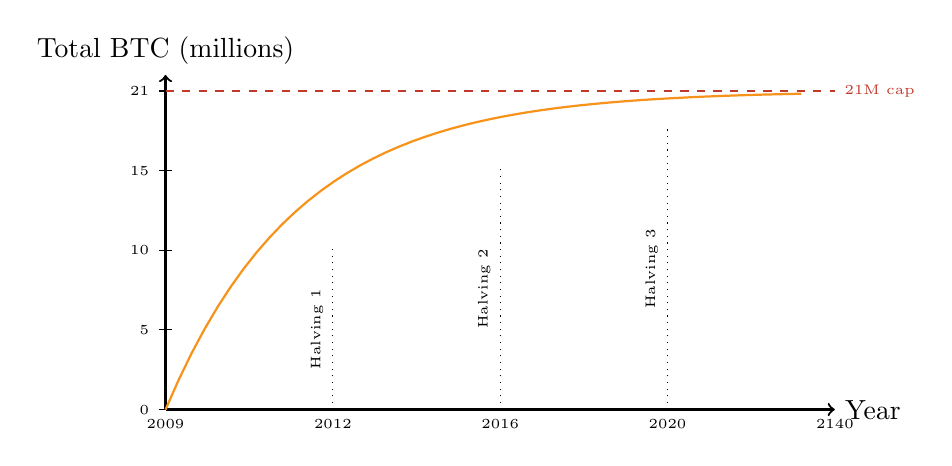
\begin{tikzpicture}[scale=0.85]
    % Axes
    \draw[thick,->] (0,0) -- (10,0) node[right] {Year};
    \draw[thick,->] (0,0) -- (0,5) node[above] {Total BTC (millions)};
    
    % Y-axis labels
    \foreach \y/\label in {0/0, 1.19/5, 2.38/10, 3.57/15, 4.76/21} {
        \draw (-0.1,\y) -- (0.1,\y);
        \node[left, font=\tiny] at (-0.1,\y) {\label};
    }
    
    % X-axis labels
    \node[below, font=\tiny] at (0,0) {2009};
    \node[below, font=\tiny] at (2.5,0) {2012};
    \node[below, font=\tiny] at (5,0) {2016};
    \node[below, font=\tiny] at (7.5,0) {2020};
    \node[below, font=\tiny] at (10,0) {2140};
    
    % Supply curve (logarithmic approach to 21M)
    \draw[thick, cryptogold, domain=0:9.5, samples=50] 
        plot (\x, {4.76*(1-exp(-0.5*\x))});
    
    % Asymptote
    \draw[dashed, cryptored] (0,4.76) -- (10,4.76);
    \node[right, font=\tiny, cryptored] at (10,4.76) {21M cap};
    
    % Halving annotations
    \draw[dotted] (2.5,0) -- (2.5,2.4);
    \draw[dotted] (5,0) -- (5,3.6);
    \draw[dotted] (7.5,0) -- (7.5,4.2);
    
    \node[above, font=\tiny, rotate=90] at (2.5,1.2) {Halving 1};
    \node[above, font=\tiny, rotate=90] at (5,1.8) {Halving 2};
    \node[above, font=\tiny, rotate=90] at (7.5,2.1) {Halving 3};
\end{tikzpicture}
\end{center}

Unlike fiat currency, Bitcoin's supply is \textbf{algorithmically fixed}. No central bank can ``print'' more. Block rewards halve every $\sim$4 years until all 21 million are mined ($\sim$2140).
\end{frame}

% Slide 16: Argument 2 - Financial Privacy
\begin{frame}{Argument 2: Financial Freedom and Privacy}
\begin{probox}[The Financial Privacy Argument]
\begin{enumerate}
    \item Financial transactions reveal intimate details about our lives
    \item Governments and corporations increasingly surveil financial activity
    \item Privacy is necessary for freedom (self-censorship under surveillance)
    \item Cash provided anonymity; digital payments eliminate it
    \item \textbf{Therefore}: Cryptocurrency restores financial privacy in the digital age
\end{enumerate}
\end{probox}

\vspace{0.3em}
\textbf{Examples}: Bank account freezes for political dissidents, ``debanking'' of controversial figures, Canadian trucker convoy (2022).

\textbf{Philosophical connection}: Money is speech; financial censorship is a form of silencing.

\begin{alertblock}{Discussion}
Where should the line between privacy and accountability be?
\end{alertblock}
\end{frame}

% Slide 17: Argument 3 - Financial Inclusion
\begin{frame}{Argument 3: Financial Inclusion (Banking the Unbanked)}
\begin{probox}[The Inclusion Argument]
\small
\begin{enumerate}
    \item $\sim$1.3 billion adults globally lack access to banking (World Bank 2025)
    \item Traditional banking has high barriers: ID, minimums, physical access
    \item Cryptocurrency requires only internet access---no bank, ID, or credit history
    \item \textbf{Therefore}: Cryptocurrency can provide financial services to the excluded
\end{enumerate}
\end{probox}

\vspace{-0.3em}
\begin{table}[h]
\centering
\scriptsize
\begin{tabular}{@{}lcc@{}}
\toprule
\textbf{Region} & \textbf{Account Ownership} & \textbf{Change since 2011} \\
\midrule
High-income & 97\% & +3\% \\
Sub-Saharan Africa & 58\% & +35\% \\
\textbf{Global} & \textbf{79\%} & \textbf{+28\%} \\
\bottomrule
\end{tabular}
\caption*{\scriptsize Source: World Bank Global Findex 2025}
\end{table}
\end{frame}

% Slide 18: Argument 4 - Protection from Overreach
\begin{frame}{Argument 4: Protection from Government Overreach}
\begin{probox}[The Anti-Tyranny Argument]
\small
\begin{enumerate}
    \item Authoritarian governments control citizens through financial systems
    \item Bank accounts can be frozen, assets seized, transactions blocked
    \item Cryptocurrency is ``censorship-resistant''---no government can stop transactions
    \item \textbf{Therefore}: Cryptocurrency protects human rights and individual liberty
\end{enumerate}
\end{probox}

\vspace{0.2em}
\textbf{Examples}: Hong Kong protesters (2019--2020), Russian dissidents, Venezuelan refugees.

\textbf{Philosophical grounding}: Property rights as human rights; economic freedom as prerequisite for political freedom.

\begin{alertblock}{Discussion}
Can a technology be both a tool for freedom fighters and criminals?
\end{alertblock}
\end{frame}

% Slide 19: Argument 5 - Decentralization
\begin{frame}{Argument 5: Decentralization as a Democratic Value}
\begin{columns}[T]
\begin{column}{0.45\textwidth}
\textbf{Centralized System}
\begin{center}
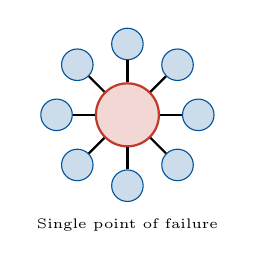
\begin{tikzpicture}[scale=0.6]
    \node[circle, draw=cryptored, fill=cryptored!20, thick, minimum size=0.8cm] (center) at (0,0) {};
    \foreach \angle in {0,45,90,135,180,225,270,315} {
        \node[circle, draw=cryptoblue, fill=cryptoblue!20, minimum size=0.4cm] (n\angle) at (\angle:1.5) {};
        \draw[thick] (center) -- (n\angle);
    }
    \node[below, font=\tiny] at (0,-2) {Single point of failure};
\end{tikzpicture}
\end{center}
\end{column}
\begin{column}{0.45\textwidth}
\textbf{Decentralized System}
\begin{center}
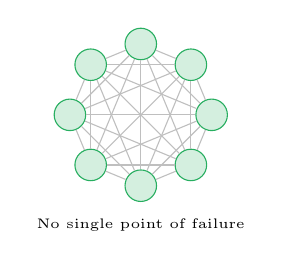
\begin{tikzpicture}[scale=0.6]
    \foreach \i in {1,...,8} {
        \pgfmathsetmacro{\angle}{(\i-1)*45}
        \node[circle, draw=cryptogreen, fill=cryptogreen!20, minimum size=0.4cm] (n\i) at (\angle:1.5) {};
    }
    \foreach \i in {1,...,8} {
        \foreach \j in {1,...,8} {
            \ifnum\i<\j
                \draw[thin, gray!50] (n\i) -- (n\j);
            \fi
        }
    }
    \node[below, font=\tiny] at (0,-2) {No single point of failure};
\end{tikzpicture}
\end{center}
\end{column}
\end{columns}

\vspace{0.5em}
\textbf{The argument}: Centralized institutions accumulate power and become corrupt. ``Too big to fail'' creates moral hazard. Decentralized systems distribute power and increase resilience.

\begin{alertblock}{Discussion}
Is decentralization always better? What are its costs?
\end{alertblock}
\end{frame}

% Slide 20: Case Study - El Salvador
\begin{frame}{Case Study: El Salvador's Bitcoin Experiment}
\begin{casestudybox}[Timeline]
\textbf{September 2021}: First country to adopt Bitcoin as legal tender.\\
\textbf{2021--2024}: Chivo wallet launched; \$30 bonus for sign-ups; mixed results.\\
\textbf{January 2025}: Bitcoin legal tender status \textbf{revoked} as condition for \$1.4B IMF loan.
\end{casestudybox}

\vspace{0.3em}
\textbf{What happened?}
\begin{itemize}
    \item By 2024, 92\% of Salvadorans did not use Bitcoin for transactions
    \item Only 1.3\% of remittances used cryptocurrency
    \item Chivo wallet plagued by technical issues, fraud, identity theft
    \item IMF demanded Bitcoin be made voluntary for loan approval
\end{itemize}

\begin{alertblock}{Lesson}
Top-down adoption failed. Trust must be earned, not mandated.
\end{alertblock}
\end{frame}

%% PART III: CRITICISMS OF PRO-CRYPTO ARGUMENTS %%
\section{Part III: Criticisms of Pro-Crypto Arguments}

% Slide 21: Critique - Deflation Problem
\begin{frame}{Critique: The Deflation Problem}
\begin{objectionbox}[Response to Sound Money Argument]
\begin{itemize}
    \item Moderate inflation serves economic purposes (encourages spending/investment)
    \item Deflation is economically dangerous (Great Depression, Japan's ``lost decades'')
    \item Fixed supply creates deflationary pressure as economy grows
    \item Hoarding incentive: Why spend if it will be worth more tomorrow?
    \item Result: Poor medium of exchange---too volatile to price goods
\end{itemize}
\end{objectionbox}

\vspace{0.3em}
\textbf{The volatility problem}: Bitcoin has lost 50\%+ of value multiple times:
\begin{itemize}
    \item 2014: $-$85\% from peak
    \item 2018: $-$84\% from peak  
    \item 2022: $-$77\% from peak
\end{itemize}

Paul Krugman: Cryptocurrency is ``a solution in search of a problem.''
\end{frame}

% Slide 22: Critique - Privacy Dark Side
\begin{frame}{Critique: The Dark Side of Privacy}
\begin{objectionbox}[Response to Privacy Argument]
\begin{itemize}
    \item Financial surveillance serves legitimate purposes (crime prevention, tax enforcement)
    \item Cryptocurrency enables: money laundering, ransomware, sanctions evasion, terrorism financing
    \item Pseudonymity $\neq$ anonymity---blockchain analysis can identify users
    \item Privacy vs. accountability: Should anyone have untraceable wealth?
\end{itemize}
\end{objectionbox}

\vspace{0.3em}
\textbf{North Korea's Lazarus Group} (2025 data):
\begin{itemize}
    \item Stole \$2.02 billion in cryptocurrency in 2025 alone
    \item Cumulative theft: \$6.75 billion since 2017
    \item Largest single heist: \$1.5 billion from Bybit (February 2025)
    \item Funds weapons and missile programs
\end{itemize}
\end{frame}

% Slide 23: Critique - Who Actually Benefits?
\begin{frame}{Critique: Who Actually Benefits from Crypto?}
\begin{objectionbox}[Response to Financial Inclusion Argument]
\begin{itemize}
    \item The unbanked often lack: internet access, smartphones, technical knowledge
    \item Volatility hurts the poor most---they can't afford to lose 50\%
    \item Complexity creates barriers; scams target unsophisticated users
    \item Transaction fees can be high during network congestion
    \item In practice, crypto adoption highest among already-banked, tech-savvy users
\end{itemize}
\end{objectionbox}

\vspace{0.3em}
\textbf{Alternative}: Mobile banking (M-Pesa), fintech apps, and traditional financial inclusion efforts may be more effective and less risky.

\textbf{Reality check}: Most crypto trading is speculation, not payments or remittances.

\begin{alertblock}{Discussion}
Does cryptocurrency help the unbanked, or mainly benefit speculators?
\end{alertblock}
\end{frame}

% Slide 24: Critique - Is It Actually Decentralized?
\begin{frame}{Critique: Is Cryptocurrency Actually Decentralized?}
\begin{objectionbox}[The ``Decentralization Theater'' Problem]
\small
\begin{itemize}
    \item \textbf{Mining concentration}: $\sim$4 mining pools control $>$50\% of Bitcoin hashrate
    \item \textbf{Wealth concentration}: $\sim$2\% of accounts hold $\sim$95\% of Bitcoin
    \item \textbf{Development centralized}: Small number of core developers make key decisions
    \item \textbf{Exchanges centralized}: Most trading on Coinbase, Binance, etc.
\end{itemize}
\end{objectionbox}

\vspace{0.2em}
\begin{center}
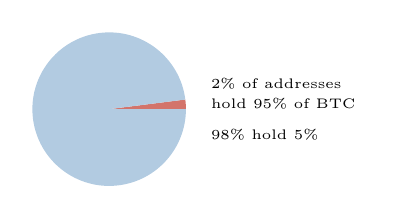
\begin{tikzpicture}[scale=0.65]
    % Pie chart showing concentration
    \fill[cryptored!70] (0,0) -- (0:1.5) arc (0:7.2:1.5) -- cycle;
    \fill[cryptoblue!30] (0,0) -- (7.2:1.5) arc (7.2:360:1.5) -- cycle;
    
    \node[font=\tiny, right] at (1.8,0.5) {2\% of addresses};
    \node[font=\tiny, right] at (1.8,0.1) {hold 95\% of BTC};
    \node[font=\tiny, right] at (1.8,-0.5) {98\% hold 5\%};
\end{tikzpicture}
\end{center}
\vspace{-0.3em}
\textbf{Governance question}: Who decides on protocol changes? (Bitcoin block size debate, Ethereum hard forks)
\end{frame}

% Slide 25: Environmental Critique
\begin{frame}{The Environmental Critique}
\begin{objectionbox}[Bitcoin's Energy Consumption (2025)]
\small
\begin{itemize}
    \item Annual electricity: $\sim$150--175 TWh (comparable to Poland or Argentina)
    \item Single transaction: $\sim$1,400+ kWh (weeks of household use)
    \item E-waste: $\sim$20,000+ tonnes annually from mining hardware
\end{itemize}
\end{objectionbox}

\vspace{-0.2em}
\begin{table}[h]
\centering
\scriptsize
\begin{tabular}{@{}lr@{}}
\toprule
\textbf{Entity} & \textbf{Annual TWh} \\
\midrule
Bitcoin network & $\sim$150--175 \\
Poland (country) & $\sim$170 \\
Google (global) & $\sim$33 \\
Ethereum (post-merge) & $\sim$0.02 \\
\bottomrule
\end{tabular}
\end{table}
\vspace{-0.3em}
\textbf{Counterargument}: Proof of Stake (Ethereum) uses 99.9\% less energy; some mining uses renewable/stranded energy.
\end{frame}

% Slide 26: Case Study - Silk Road
\begin{frame}{Case Study: Silk Road and Ross Ulbricht}
\begin{casestudybox}[The Dark Web Marketplace]
\small
\textbf{Silk Road} (2011--2013): First major dark web marketplace using Bitcoin. Primarily drugs, also forged documents and hacking services.
\end{casestudybox}

\vspace{0.2em}
\textbf{Ross Ulbricht} (``Dread Pirate Roberts''):
\begin{itemize}
    \item Libertarian philosophy: ``victimless crimes'' shouldn't be crimes
    \item Arrested October 2013; convicted February 2015; life sentence
    \item \textbf{Pardoned by President Trump in January 2025}
\end{itemize}

\textbf{Significance}: Demonstrated Bitcoin's use for illegal activity; shaped early public perception.

\begin{alertblock}{Philosophical Question}
Does enabling criminal activity invalidate the technology, or is it a feature (like cash)?
\end{alertblock}
\end{frame}

%% PART IV: THE CASE FOR REGULATION %%
\section{Part IV: The Case FOR Regulation}

% Slide 27: The Dominant View
\begin{frame}{The Dominant View: Why Most Experts Are Skeptical}
Cryptocurrency skeptics include most academic economists, central bankers, securities regulators, and many technologists.

\vspace{0.3em}
\textbf{Key concerns}: Consumer protection, financial stability, crime facilitation, environmental harm.

\begin{quotebox}
``Whether it goes up or down... I'm pretty sure of is that it doesn't produce anything.''\\
\hfill---Warren Buffett
\end{quotebox}

\begin{quotebox}
``In my life, I try to avoid things that are stupid and evil and make me look bad... and bitcoin does all three.''\\
\hfill---Charlie Munger (2022)
\end{quotebox}

Nobel laureates critical of crypto: Paul Krugman, Joseph Stiglitz, Robert Shiller.
\end{frame}

% Slide 28: Argument 1 - Consumer Protection
\begin{frame}{Argument 1: Consumer Protection}
\begin{argumentbox}[The Consumer Protection Argument]
\begin{enumerate}
    \item Most retail investors lack technical knowledge to evaluate crypto
    \item The space is rife with fraud, scams, and manipulation
    \item ``Pump and dump'' schemes, rug pulls, fake projects are endemic
    \item Volatility causes devastating losses for unsophisticated investors
    \item \textbf{Therefore}: Regulation is necessary to protect ordinary people
\end{enumerate}
\end{argumentbox}

\vspace{0.3em}
\textbf{Examples of fraud}:
\begin{itemize}
    \item BitConnect (Ponzi scheme, 2018): \$2.5 billion lost
    \item OneCoin (2014--2017): \$4+ billion defrauded
    \item Countless ``rug pulls'' where developers abandon projects with funds
\end{itemize}

\textbf{FOMO psychology}: Social media hype drives irrational investment.
\end{frame}

% Slide 29: Argument 2 - Financial Stability
\begin{frame}{Argument 2: Financial Stability}
\begin{argumentbox}[The Systemic Risk Argument]
\begin{enumerate}
    \item Crypto markets are increasingly connected to traditional finance
    \item Large-scale crypto collapse could spread contagion
    \item Stablecoins create ``shadow banking'' risks without regulation
    \item Leverage and derivatives amplify risks
    \item \textbf{Therefore}: Crypto threatens broader financial stability
\end{enumerate}
\end{argumentbox}

\vspace{0.3em}
\textbf{Example}: Terra/Luna collapse (May 2022)---\$40--60 billion evaporated in days.

\textbf{Stablecoin risk}: If confidence breaks, rapid liquidation could crash markets (like a bank run, but faster).

\textbf{Historical parallel}: 2008 financial crisis began with unregulated financial instruments (CDOs, CDS).
\end{frame}

% Slide 30: Argument 3 - Enabling Crime
\begin{frame}{Argument 3: Enabling Crime}
\begin{argumentbox}[The Criminal Enablement Argument]
Cryptocurrency is the preferred payment for ransomware, darknet markets, money laundering, and sanctions evasion. Cross-border, instant, irreversible transactions defeat law enforcement.
\end{argumentbox}

\vspace{-0.2em}
\begin{table}[h]
\centering
\scriptsize
\begin{tabular}{@{}lrl@{}}
\toprule
\textbf{Year} & \textbf{N. Korea Theft} & \textbf{Notable Incident} \\
\midrule
2022 & \$1.7 billion & Ronin Bridge (\$620M) \\
2023 & \$660 million & Multiple exchanges \\
2024 & \$1.3 billion & DMM Bitcoin (\$308M) \\
2025 & \$2.02 billion & Bybit (\$1.5B) \\
\midrule
\textbf{Total} & \textbf{\$6.75 billion} & Funds weapons programs \\
\bottomrule
\end{tabular}
\caption*{\scriptsize Source: Chainalysis 2025}
\end{table}
\vspace{-0.5em}
{\small \textbf{Key Point}: State-sponsored hackers funding nuclear weapons development.}
\end{frame}

% Slide 31: Argument 4 - Greater Fool Theory
\begin{frame}{Argument 4: The ``Greater Fool'' Theory}
\begin{argumentbox}[The Speculative Bubble Argument]
\small
\begin{enumerate}
    \item Cryptocurrency has no intrinsic value (produces nothing, pays no dividends)
    \item Value depends entirely on finding someone to pay more later
    \item Eventually, greater fools run out---bubble bursts
    \item \textbf{Therefore}: Cryptocurrency is not a legitimate asset class
\end{enumerate}
\end{argumentbox}

\vspace{0.2em}
\begin{quotebox}
\small
``If you told me you own all of the bitcoin in the world and you offered it to me for \$25, I wouldn't take it because what would I do with it?''\\
\hfill---Warren Buffett (2022)
\end{quotebox}

\textbf{The tulip analogy}: Speculative manias are nothing new (Dutch tulip mania, 1637).
\end{frame}

% Slide 32: Argument 5 - Tax Evasion
\begin{frame}{Argument 5: Regulatory Arbitrage and Tax Evasion}
\begin{argumentbox}[The Democratic Governance Argument]
\begin{enumerate}
    \item Cryptocurrency enables moving wealth outside legal frameworks
    \item Tax evasion deprives societies of resources for public goods
    \item Regulatory arbitrage undermines labor, environmental, consumer protections
    \item ``If you can't beat them, join them''---regulatory race to the bottom
    \item \textbf{Therefore}: Cryptocurrency undermines democratic governance
\end{enumerate}
\end{argumentbox}

\vspace{0.3em}
\textbf{Philosophical point}: Oliver Wendell Holmes Jr.: ``Taxes are the price we pay for a civilized society.''

Tax evasion = free-riding on public goods others pay for.

\begin{alertblock}{Discussion}
Is avoiding taxes through crypto different from using offshore accounts or other tax havens?
\end{alertblock}
\end{frame}

% Slide 33: Case Study - FTX
\begin{frame}{Case Study: The FTX Collapse and Sam Bankman-Fried}
\begin{casestudybox}[The Rise and Fall]
\textbf{Sam Bankman-Fried}: MIT physics graduate, ``effective altruist,'' crypto wunderkind.\\
\textbf{FTX}: Founded 2019, grew to \$32 billion valuation, celebrity endorsements (Tom Brady, Larry David).
\end{casestudybox}

\vspace{0.3em}
\textbf{The collapse} (November 2022): Customer funds misappropriated to sister company Alameda Research. At least \$8 billion in customer funds stolen.

\textbf{Legal outcome}:
\begin{itemize}
    \item Convicted November 2023 on 7 counts of fraud
    \item \textbf{Sentenced March 28, 2024 to 25 years in prison}
    \item Ordered to forfeit \$11 billion
\end{itemize}

Judge Kaplan: ``There was a risk that this man will be in a position to do something very bad in the future, and it's not a trivial risk.''
\end{frame}

% Slide 34: Case Study - Terra Luna
\begin{frame}{Case Study: Terra/Luna and Do Kwon}
\begin{casestudybox}[Algorithmic Stablecoin Failure]
\small
\textbf{Terra/Luna}: UST ``stablecoin'' maintained \$1 peg through algorithmic arbitrage with LUNA token---no actual reserves.\\
\textbf{Do Kwon}: Founder, known for dismissing critics as ``poor.''
\end{casestudybox}

\vspace{0.2em}
{\small \textbf{The collapse} (May 2022): UST lost its peg, triggering ``death spiral.'' \$40--60 billion destroyed in days. Triggered cascade affecting Celsius, Three Arrows Capital, FTX.}

\textbf{Aftermath}:
\begin{itemize}
    \item Do Kwon arrested March 2023 in Montenegro with fake passport
    \item \textbf{Sentenced December 2025 to 15 years in prison}
\end{itemize}

\begin{alertblock}{Lesson}
``Algorithmic'' doesn't mean safe. Confidence can evaporate instantly.
\end{alertblock}
\end{frame}

%% PART V: CRITICISMS OF REGULATION ARGUMENTS %%
\section{Part V: Criticisms of Regulation Arguments}

% Slide 35: Critique - Traditional Finance Problems
\begin{frame}{Critique: Traditional Finance Also Has Problems}
\begin{objectionbox}[Response to Regulation Arguments]
\small
\begin{itemize}
    \item 2008 crisis was caused by \emph{regulated} banks, not crypto
    \item HSBC, Deutsche Bank laundered billions for cartels---small fines, no executives jailed
    \item Fraud exists everywhere; crypto is just newer
    \item ``Illicit use'' is small percentage of crypto transactions ($\sim$0.5--1\%)
\end{itemize}
\end{objectionbox}

\vspace{0.2em}
\textbf{The double standard}: Why hold crypto to higher standard than traditional finance?

\textbf{Counter}: Two wrongs don't make a right. ``Traditional finance is bad'' doesn't make crypto good.

\begin{alertblock}{Discussion}
Should we compare crypto to an ideal financial system, or to the actual one we have?
\end{alertblock}
\end{frame}

% Slide 36: Critique - Innovation Argument
\begin{frame}{Critique: Innovation Requires Permissionless Experimentation}
\begin{objectionbox}[Response to Precautionary Regulation]
\begin{itemize}
    \item Early internet faced similar criticisms (fraud, illegal content, etc.)
    \item Premature regulation would have killed transformative technology
    \item Regulators often don't understand the technology they're regulating
    \item Innovation happens at the margins; regulation protects incumbents
    \item Some beneficial uses only emerge through experimentation
\end{itemize}
\end{objectionbox}

\vspace{0.3em}
\textbf{Historical examples}: SEC was initially hostile to money market funds, ATMs, online trading---all now mainstream.

\textbf{Counter}: Crypto has had 15+ years. What beneficial uses have emerged beyond speculation?

\begin{alertblock}{Discussion}
How long should we wait before regulating a potentially harmful technology?
\end{alertblock}
\end{frame}

% Slide 37: Critique - Regulatory Capture
\begin{frame}{Critique: Regulatory Capture and Incumbent Protection}
\begin{objectionbox}[Response to ``Expert Consensus'']
\begin{itemize}
    \item Central bankers have obvious interest in maintaining monetary monopoly
    \item Banks have obvious interest in blocking competition
    \item ``Experts'' failed to predict 2008 crisis---why trust them on crypto?
    \item Regulatory capture: Industries often control their regulators
    \item CBDCs may be the real agenda---total financial surveillance
\end{itemize}
\end{objectionbox}

\vspace{0.3em}
\textbf{Public choice theory}: Regulators act in their own interest, not public interest.

\textbf{Counter}: Expertise matters. Populist distrust of experts is itself dangerous.

\begin{alertblock}{Discussion}
How do we distinguish legitimate expertise from self-interested gatekeeping?
\end{alertblock}
\end{frame}

% Slide 38: Critique - International Coordination
\begin{frame}{Critique: The International Coordination Problem}
\begin{objectionbox}[Response to National Regulation]
\begin{itemize}
    \item Cryptocurrency is global; national regulation is limited
    \item Harsh regulation just pushes activity offshore
    \item Regulatory arbitrage: Projects relocate to friendly jurisdictions
    \item Prohibition doesn't work (alcohol, drugs, etc.)
    \item Better to regulate and engage than ban and lose oversight
\end{itemize}
\end{objectionbox}

\vspace{0.3em}
\textbf{Example}: China banned crypto mining in 2021; miners moved to US, Kazakhstan, Russia. Adoption continued globally.

\textbf{The challenge}: How to regulate a borderless technology with bordered governments?

\begin{alertblock}{Discussion}
Is crypto more like the internet (hard to regulate) or like banking (heavily regulated)?
\end{alertblock}
\end{frame}

%% PART VI: THE FUTURE AND CONCLUSION %%
\section{Part VI: The Future and Conclusion}

% Slide 39: CBDCs
\begin{frame}{Central Bank Digital Currencies (CBDCs)---A Middle Path?}
\textbf{CBDCs}: Digital currency issued by central banks. Adopts crypto's technology while rejecting its philosophy.

\vspace{0.2em}
\begin{table}[h]
\centering
\footnotesize
\begin{tabular}{@{}llp{5cm}@{}}
\toprule
\textbf{Country} & \textbf{Status} & \textbf{Notes} \\
\midrule
Bahamas & Launched (2020) & Sand Dollar---first CBDC \\
Jamaica & Launched (2022) & JAM-DEX \\
China & Pilot & e-CNY: 260M wallets, 7T yuan in transactions \\
EU & Preparation & Digital Euro in development \\
\textbf{USA} & \textbf{Banned} & Trump executive order (Jan 2025) \\
\bottomrule
\end{tabular}
\caption*{\footnotesize Source: Atlantic Council CBDC Tracker (134 jurisdictions exploring)}
\end{table}

\textbf{Potential benefits}: Financial inclusion, payment efficiency, monetary policy tools.

\textbf{Concerns}: \textbf{Total financial surveillance}, programmable restrictions, negative interest rates.
\end{frame}

% Slide 40: Conclusion
\begin{frame}{Conclusion: Evaluating Cryptocurrency Ethically}
\textbf{Key tensions to weigh:}
\begin{itemize}
    \item \textbf{Privacy vs. Accountability}: Where should the line be?
    \item \textbf{Innovation vs. Protection}: How to balance experimentation with preventing harm?
    \item \textbf{Freedom vs. Stability}: Individual liberty vs. collective security?
    \item \textbf{Decentralization vs. Governance}: Who makes rules in a decentralized system?
\end{itemize}

\vspace{0.3em}
\textbf{Framework for evaluation}: Who benefits? Who is harmed? What are the alternatives? What values are at stake? What does the evidence show?

\vspace{0.3em}
\begin{center}
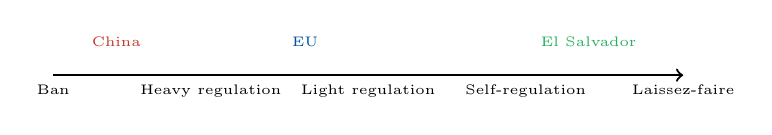
\begin{tikzpicture}[scale=0.8]
    \draw[thick, ->] (0,0) -- (10,0);
    \node[below, font=\tiny] at (0,0) {Ban};
    \node[below, font=\tiny] at (2.5,0) {Heavy regulation};
    \node[below, font=\tiny] at (5,0) {Light regulation};
    \node[below, font=\tiny] at (7.5,0) {Self-regulation};
    \node[below, font=\tiny] at (10,0) {Laissez-faire};
    
    \node[above, font=\tiny, cryptored] at (1,0.3) {China};
    \node[above, font=\tiny, cryptoblue] at (4,0.3) {EU};
    \node[above, font=\tiny, cryptogreen] at (8.5,0.3) {El Salvador};
\end{tikzpicture}
\end{center}

\begin{alertblock}{Final Discussion}
After considering all arguments, what's your view? Should crypto be banned, regulated, or left alone?
\end{alertblock}
\end{frame}

\end{document}